\documentclass[a4paper, 12pt]{article}
\setcounter{secnumdepth}{0}

\usepackage{epigraph}

\usepackage[portuges]{babel}
\usepackage[utf8]{inputenc}
\usepackage{amsmath}
\usepackage{indentfirst}
\usepackage{graphicx}
\usepackage{multicol,lipsum}
\usepackage{caption}
\usepackage{listings}
\usepackage{subcaption}
\usepackage{biblatex}

\setcounter{tocdepth}{5}
\setcounter{secnumdepth}{5}

\usepackage{hyperref}
\hypersetup{
    colorlinks,
    citecolor=black,
    filecolor=black,
    linkcolor=black,
    urlcolor=black
}

\newtheorem{definition}{Definição}[section]
\newtheorem{remark}{Observação}

\title{Mecânica e Ondas\\ \Large{Sebenta de Apoio ao Estudo}}
\author{Carlos Menezes}
\date{4 de maio de 2021}

\begin{document}

\maketitle

\newpage

\tableofcontents

\newpage
\newpage

\part{Cinemática e Dinâmica}

\newpage

\section{Forças}
\subsection{Conteúdo Importante}
\subsubsection{Primeira Lei de Newton}

Com as Leis de Newton, começamos o estudo de como o movimento ocorre no mundo real. O estudo das causas do movimento é chamado de dinâmica ou mecânica. A relação entre força e a aceleração foi dada por Isaac Newton em suas três leis do movimento, que formam o base da física elementar. Embora a formulação da física de Newton tivesse que ser substituída mais tarde, para lidar com o movimento em velocidades comparáveis à velocidade da luz e para o movimento no escala de átomos, é aplicável a situações cotidianas e ainda é a melhor introdução para as leis fundamentais da natureza. O estudo das leis de Newton e suas implicações é muitas vezes chamada de mecânica newtoniana ou clássica.

As partículas aceleram porque sofrem ação de forças. Na ausência de forças, uma partícula não acelera, movendo-se com uma velocidade constante.

\begin{definition}[Primeira Lei de Newton.] Considerando um corpo no qual não hã ação de forças. Então, se esse mesmo corpo estiver em repouso, permanecerá em repouso, e se estiver se movendo com velocidade constante, continua a mover-se nessa velocidade.
\end{definition}

\subsubsection{Segunda Lei de Newton}
Experiencias demonstram que os objetos têm uma propriedade chamada \textbf{massa} que mede como o seu movimento é influenciado por forças. A Segunda Lei de Newton é uma relação entre a \textbf{força resultante} ($F$) agindo sobre uma massa $m$ e sua aceleração $a$.

\begin{definition}[Segunda Lei de Newton] $\sum F=ma$
\end{definition}

A relação acima é uma relação \emph{vetorial}, pelo que em duas dimensões, esta equação implica:

\begin{equation}\label{eqn:2newton}
    \sum F_x=ma_x \qquad \sum F_y=ma_y
\end{equation}

A unidade de força no SI é $kg\ ms^{-2}$, abreviada em newton ($N$). Deste modo,

\begin{equation*}
    1\ newton = 1 N = 1\ kg\ ms^{-2}
\end{equation*}

\subsubsection{Exemplos de Forças}
A Terra exerce uma força gravitacional com sentido para baixo em todas as massas perto da sua superfície. Esta força é conhecida como o \textbf{peso}, $F_g$, e a sua magnitude é dada por

\begin{equation}
    F_g=mg    
\end{equation}

Uma corda sob tensão exerce uma força nos objetos que estão apensos em cada uma das pontas. As forças estão direcionadas para dentro ao longo do comprimento da corda. A tensão é simbolizada pela letra $T$.

Uma superfície sólida exerce uma força em qualquer massa com a qual esteja em contacto. De modo geral, a força da superfície terá uma componente perpendicular/normal, denominada \textbf{força normal} da superfície. A superfície pode também exercer uma força paralela: a força de fricção.

\subsubsection{Terceira Lei de Newton}
Esta lei é popularmente enunciada como "lei da ação-reação", mas na verdade lida com as forças entre dois objetos.

\begin{definition}[Terceira Lei de Newton.] Considerando dois objetos A e B. A força que o objeto A exerce no objeto B é igual e oposta à força que o objeto B exerce no objeto A: $F_{AB}=-F_{BA}$
\end{definition}

\subsubsection{Aplicação das Lei de Newton}
Uma dica útil apra problemas que envolvem mais do que uma força é desenhar um diagrama que evidencia as massas individuais no problema, juntamento com os vetores que mostram as direções e magnitudes das forças individuais. A estes diagramas é dado o nome de \textbf{diagramas de corpo-livre}.

\subsubsection{Atrito}
Forças que são conhecidas coletivamente como “forças de atrito” estão ao nosso redor na vida diária. Na física elementar, discutimos a força de atrito conforme ela ocorre entre dois objetos cujas
superfícies estão em contato e deslizam uma contra a outra. Se, em tal situação, um corpo não se mover enquanto uma força $F$ age sobre ele, então
as forças de \textbf{atrito estático} opõem-se à força $F$, pelo que a força resultante será zero. Empiricamente,
descobre-se que esta força pode ter um valor máximo dado por:

$$
f_s^{max}=\mu_sN
$$

onde $\mu_s$ é o \textbf{coeficiente de atrito estático} para as duas superfícies e $N$ é a força normal entre as duas.
Se um objeto está em movimento em relação a outro, então existe uma força de \textbf{atrito cinético} entre os dois objetos. A direção desta força é tal que se opõe ao movimento e a sua magnitude é dada por

$$
f_k=\mu_kN
$$

onde $N$ é a força normal entre os objetos e $\mu_k$ o \textbf{coeficiente de atrito cinético} para as duas superfícies.

\subsubsection{Revisitando o Movimento Circular Uniforme}

Como visto em capítulos anteriores, quand oum objeto está em movimento circular uniforme, movendo-se em forma de círculo de raio \emph{r} com velocidade \emph{v}, a aceleração (centrípeta) é dirigida para o centro do círculo e tem magnitude

\begin{equation}
    a_{c}=\frac{v^2}{r}
\end{equation}

Desta maneira, da Segunda Lei de Newton, a força resultante que atua neste objeto tem também de ser direcionada para o centro da trajetória e ter magnitude

\begin{equation}
    F_{c}=\frac{mv^2}{r}
\end{equation}

Tal força é chamada \textbf{força centrípeta}.

\subsubsection{Lei da Gravitação Universal}
A força gravítica é uma das forças fundamentais da natureza. Todas as massas exercem uma força gravitacional atrativa umas sobre as outras, mas para a maioria dos objetos a força é tão pequena que podemos ignorá-la.

A Lei da Gravitação Universal diz que para duas massas $m_1$ e $m_2$, separadas por uma distância $r$, a magnitude da força gravitacional é

\begin{equation}\label{eq:lei_da_gravidade}
    F=G\frac{m_1m_2}{r^2} \qquad onde \qquad G=6.67\times 10^{-11}\frac{N\cdot m^2}{kg^2}
\end{equation}

% \section{Exercícios}
% \subsection{Segunda Lei de Newton}
\textbf{1.} Uma massa de 3.0kg sofre uma aceleração dada por $a=(2.0i + 5.0j)ms^{-2}$. Qual é a força resultante e a sua magnitude?
\linebreak
A Segunda Lei de Newton diz-se que a força resultante numa massa $m$ é $\sum F = ma$. Portanto,

$$
\begin{aligned}
    F_{R}&=ma \\
        &=(3.0\ kg)(2.0i+5.0j)ms^{-2} \\
        &=(6.0i + 15j)N
\end{aligned}
$$

A magnitude da $F_{R}$ é dada pelo cálculo da norma do vetor $F_{R}$:

$$
\begin{aligned}
    F_{R}=\sqrt{(6.0N)^2+(15.0N)^2}=16N
\end{aligned}
$$

\textbf{2.} Enquanto duas forças agem sobre ela, uma massa de $m=3.2kg$ move-se com uma velocidade constante $(3ms)i-(4ms)j$. Uma dessas forças é $F_1=(2N)i+(-6N)j$. Qual é a outra força?
\linebreak
A Segunda Lei de Newton diz-se que a força resultante numa massa $m$ é $\sum F = ma$. Portanto, $\sum F = ma \equiv F_1+F_2=ma$. Neste caso, a velocidade é constante, pelo que $a=0$. Portanto,

$$
\begin{aligned}
    F_1+F_2&=0 \\
    \implies F_2&=-F_1 \\
    \implies F_2&=-[(2N)i+(-6N)j] \\
    \implies F_2&=(-2N)i+(6N)j
\end{aligned}
$$

\textbf{3.} Um objeto de massa $m=4.0\ kg$ tem uma velocidade de $3.0i\ ms^{-1}$ num dado instante. Oito segundos depois, a sua velocidade é $(8.0i+10.0j)ms^{-1}$. Assumindo que o objeto foi sujeito a uma força resultante constante, encontre (a) as componentes da força e (b) a sua magnitude. \\
\linebreak
\textbf{(a)} É-nos dito que a força resultante que age na massa foi constante. Logo, sabemos que a sua aceleração foi igualmente constante, we podemos usar resultados de capítulos anteriores. São facultadas as velocidades inicias e final, pelo que é possível calcular as componentes da aceleração:

$$
a_x=\frac{\Delta v_x}{\Delta t}=\frac{[(8.0\ ms^{-1})-(3.0\ ms^{-1})]}{(8.0\ s)}=0.63\ ms^{-2}
$$

$$
a_y=\frac{\Delta v_y}{\Delta t}=\frac{[(1.0\ ms^{-1})-(0.0\ ms^{-1})]}{(8.0\ s)}=1.3\ ms^{-2}
$$

Visto que a massa é facultada no enunciado, é possível calcular as componentes da força resultante:

$$
\begin{aligned}
    F_x=ma_x=(4.0\ kg)(0.63\ ms^{-2})=2.5N \\
    F_y=ma_y=(4.0\ kg)(1.3\ ms^{-2})=5.0N \\
\end{aligned}
$$

\textbf{(b)} A magnitude da força resultante é obtida através da seguinte computação:

$$
F=\sqrt{F_x^2+F_y^2}=\sqrt{(2.5\ N)^2+(5.0\ N)^2}=5.6\ N
$$

A direção $\theta$ da força $F$ é dada por

$$
\tan \theta = \frac{F_y}{F_x} = 2.0 \quad \implies \quad \theta = \arctan(2.0)=63.4^{\circ}
$$

\textbf{4.} Cinco forças atuam sobre a caixa de massa $4.0\ kg$ na Figura \ref{fig:4caixa}. Encontre a aceleração da caixa (a) na notação unidade-vetor e (b) a sua magnitude e direção.
\linebreak
\begin{figure}[h!]
    \centering
    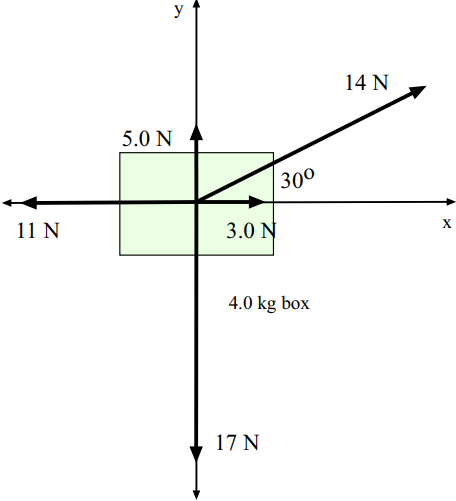
\includegraphics[width=0.5\textwidth]{forças/fig/ex4.png}
    \caption{Cinco forças atuam num caixa de massa $4.0\ kg$.}
    \label{fig:4caixa}
\end{figure}


\textbf{(a)} Existe a necessidade de separar as forças nas suas duas componentes $x$ e $y$. A Segunda Lei de Newton será utilizada para computar o valor da aceleração da caixa.

$$
\begin{aligned}
    \sum F_x&=-11N+3N+14\cos(30º) \\
    &=4.1N
\end{aligned}
$$

$$
\begin{aligned}
    \sum F_y&=+5N-17N+14\sin(30) \\
    &=-5.0N
\end{aligned}
$$

Logo, tem-se que a força resultante é

$$
\sum F=(4.1N)i+(-5.0N)j
$$

Utilizando a Equação \ref{eqn:2newton}, temos:

$$
    \sum a_x=\frac{\sum F_x}{m}=\frac{(4.1\ N)}{4.0\ kg}=1.0\ ms^{-2} \\
    \sum a_y=\frac{\sum F_y}{m}=\frac{(-5.0\ N)}{4.0\ kg}=-1.2\ ms^{-2} \\
$$


O valor da aceleração em notação vetorial é, então,

$$
a=(1.0i-1.2j)ms^{-2}
$$

\textbf{(b)} A aceleração encontrada em (a) tem magnitude

$$
a=\sqrt{a_x^2+x_y^2}=\sqrt{(4.0\ ms^{-2})^2+(-1.2\ ms^{-2})^2}=1.6\ ms^{-2}
$$

A direção $\theta$ do vetor aceleração é dada por

$$
\tan \theta = \frac{a_y}{a_x} = -1.2 \quad \implies \quad \theta = \arctan(-1.2)=-50^{\circ}
$$

Neste caso, tendo em conta que $a_y$ é negativo e $a_x$ é positivo, a escolha de $\theta = -50^{\circ}$ está correta.

\subsection{Exemplos de Forças}
\textbf{5.} Encontre a tensão em cada uma das cordas da Figura \ref{fig:5caixa}.
\linebreak
\begin{figure}[h!]
    \centering
    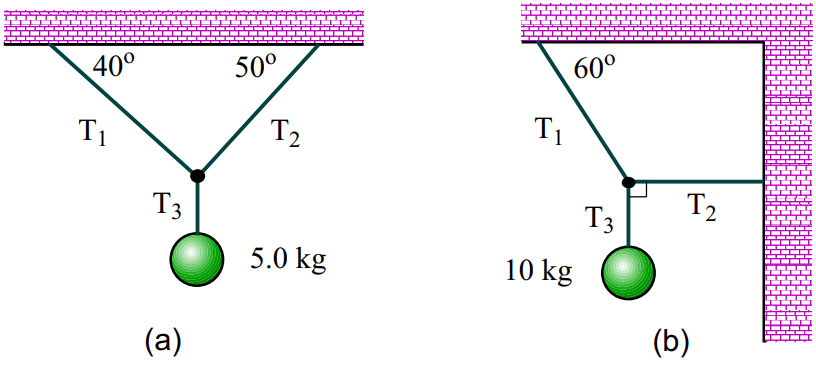
\includegraphics[width=0.5\textwidth]{forças/fig/ex5.png}
    \caption{Massas suspensas por cordas.}
    \label{fig:5caixa}
\end{figure}

\textbf{(a)} Seja $m_1$ a massa correspondente à bola representada na Figura \ref{fig:5caixa} (a). A força gravítica atua para baixo com uma força de magnitude $m_1g$. A corda vertical puxa "para cima" com uma força de magnitude $T_3$. Tendo em conta que a massa pendurada não tem aceleração, verifica-se que $T_3=m_1g$. Portanto, o valor de $T_3$ é dado por:

$$
T_3=m_1g=(5.0\ kg)(9.9\ ms^{-2})=49\ N
$$

Considerando agora o ponto de união das três cordas. Esse ponto não tem qualquer aceleração, pelo que o resultado da força resultante deverá ser zero. As componentes verticais e horizontains dessas forças somam a zero, separadamente.

$$
    \begin{cases}
        -T_1\cos(40^{\circ})+T_2\cos(50^{\circ})=0 \\
        T_1\sin(40^{\circ})+T_2\sin(50^{\circ})-T_3=0
    \end{cases}
$$

A primeira equação, a soma das componentes horizontais, dá-nos $T_2=1.19T_1$.

A segunda equação,  a soma das componentes verticais, dá-nos o valor  $T_1=31.5\ N$.

Sabendo o valor de $T_1$, $T_2=1.19T_1\ \implies \ T_2=37.5\ N$

As tensões no sistema (a) são, portanto:

$$
T_1=31.5\ N \qquad T_2=37.5\ N \qquad T_3=49\ N
$$

\textbf{(b)} A força resultante na massa pendurada, $m_2$, tem de ser 0, porque não há aceleração. Visto que a gravida "puxa para baixo" com uma força $m_2g$ e a corda vertical "puxa para cima" com uma força $T_3$, sabemos que

$$
T_3-F_g=0 \implies T_3=F_g \implies T_3=m_2g \\
\begin{aligned}
    T_3&=m_2g
    &=(10\ kg)\cdot(9.8\ ms^{-2})=98\ N
\end{aligned}
$$

Considerando agora as forças que atuam no ponto onde todas as forças se encontram. Novamente, como não há aceleração nesse ponto, tanto as componentes verticais como horizontais somam a zero.

No que toca às forças horizontais, temos:

$$
-T_1\cos(60^{\circ})+T_2=0 \qquad \implies \qquad T_2=T_1\cos(60^{\circ}) \\
$$

A soma das forças verticais é dada por:

$$
T_1\sin(60^{\circ})-T_3=0 \qquad \implies \qquad T_1=\frac{T_3}{\sin(60^{\circ})}=113\ N
$$

Podemos, depois, obter $T_2$:

$$
T_2=T_1\cos(60^{\circ})=(133\ N)\cos(60^{\circ})=56.6\ N
$$

As tensões no sistema (b) são, portanto:

$$
T_1=133\ N \qquad T_2=56.6\ N \qquad T_3=98\ N
$$

\textbf{6.} Um bloco de massa $m=2.0\ kg$ está suspenso em equilíbrio num encosta que faz um ângulo $\theta=60^{\circ}$ pela força horizontal $F$, como mostrado na Figura \ref{fig:6plano}. (a) Determine o valor de $F$, a magnitude de $F$. (b) Determine a força normal exercida pelo plano inclinado no bloco (ignore o atrito).
\linebreak
\begin{figure}[h!]
    \centering
    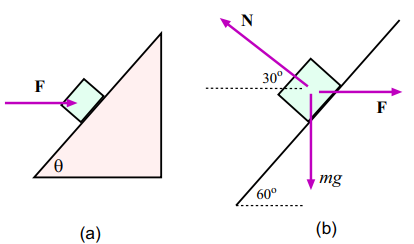
\includegraphics[width=0.5\textwidth]{forças/fig/ex6.png}
    \caption{(a) Bloco em repouso numa rampa sem atrito por uma força horizontal. (b) Forças a atuarem no bloco.)}
    \label{fig:6plano}
\end{figure}

\textbf{(a)} Fazer um diagrama de das forças que atuam no corpo torna-se essencial para este problema, daí a inclusão da \ref{fig:6plano} (b). Muitas vezes, para problemas envolvendo um bloco num plano inclinado, é mais fácil usar as componentes da $F_g$ ao longo desse mesmo plano inclinado e perpendicular a ele. Para este problema, isso não torna as coisas mais fáceis, uma vez que não há movimento no plano inclinado.

Do enunciado, retira-se a informação de que o block está em equilíbrio, pelo que não tem aceleração e as forças que em si atuam somam a zero. Este facto permite-nos escrever:

$$
N\sin(30^{\circ})-F_g=0 \qquad \implies \qquad N=\frac{F_g}{\sin(30^{\circ})}
$$

$$
N=\frac{(2.0\ kg)\cdot(9.8\ ms^{-2})}{\sin(30^{\circ})}=39.2\ N
$$

O resultado da força resultante horizontal também é nulo, logo podemos escrever:

$$
F-N\cos(30^{\circ})=0 \qquad \implies \qquad F=N\cos(30^{\circ})=33.9\ N
$$

\textbf{(b)} O resultado da força Normal foi encontrado anteriormente, $N=39.2\ N$.

\newpage

\section{Trabalho, Energia Cinética e Energia Potencial}
\subsection{Conteúdo Importante}
\subsubsection{Energia Cinética}

Para um objeto com massa $m$ e velocidade $v$, a energia cinética está definida como

\begin{equation}
    K=\frac{1}{2}mv^2
\end{equation}

A energia cinética é um escalar (tem magnitude mas não direção); é sempre um número positivo; e tem unidades do SI de $kg\cdot m^2s^{-2}$. Esta combinação é também conhecida como \textbf{joule}:

\begin{equation}
    1\ joule=1J=1\ kg\cdot m^2s^{-2}
\end{equation}

\subsubsection{Trabalho}
Quando um objeto se move enquanto um força é exercida sobre ele, então há \textbf{trabalho} a ser feito no objeto pela força.
Se um objeto efetuar um deslocamento $d$ enquanto uma \emph{força constante} \textbf{F} atua nele, a força faz uma quantidade de trabalho igual a

$$
W=F\cdot d=Fdcos\phi
$$

onde $\phi$ é o ângulo entre \textbf{d} e \textbf{F}. O trabalho é também uma grandeza escalar cujas unidades são $N\cdot m$.

O trabalho pode ser negativo; isto acontece quando o ângulo entre a força e o deslocamento é maior que $90^{\circ}$. Também pode ser \emph{zero}; isto acontece se $\phi=90^{\circ}$. Para que exista trabalho, a força tem de ter uma componente ao longo (ou oposta) à direção do deslocamento.
Se várias forças (constantes) atuarem na massa enquanto se move ao longo de um deslocamento \textbf{d}, podemos falar do \textbf{trabalho resultante} feito pelas forças,

$$
\begin{aligned}
    W_{R}&=F_1\cdot d+F_2\cdot d+F_3\cdot d...+F_n\cdot d\\
    &=(\sum F)\cdot d \\
    &=F_{R}\cdot d
\end{aligned}
$$

Se a força que atua sobre o objeto não é constante enquanto o objeto se move, então devemos calcular um integral para encontrar o trabalho realizado.
Supondo que o objeto se mova ao longo de uma linha reta (digamos, ao longo do eixo $x$, de $x_i$ a $x_f$) enquanto
uma força cujo componente $x$ é $F_x(x)$ atua sobre ele. (Ou seja, conhecemos a força $F_x$ como uma função
de $x$.) Então, o trabalho realizado é

\begin{equation}\label{eq:trabalho}
    W=\int_{x_i}^{x_f}F_x(x)dx
\end{equation}

Finalmente, podemos dar a expressão general para o trabalho feito por uma força. Se um objeto se move de $r_i=x_ii+y_ij+z_ik$ a $r_f=x_fi+y_fj+z_fk$ enquanto a força $F(r)$ atua sobre ele, o trabalho feito é:

\begin{equation}
    W=\int_{x_i}^{x_f}F_x(r)dx+\int_{y_i}^{y_f}F_y(r)dy+\int_{z_i}^{z_f}F_z(r)dz
\end{equation}

onde os integrais são calculados ao longo do caminho traçado pelo objeto. Esta expressão pode ser abreviada por

\begin{equation}
W=\int_{r_i}^{r_f}F\cdot dr
\end{equation}

A gravidade funciona em objetos que se movem verticalmente. Pode-se mostrar que se a altura de um objeto mudou numa quantidade $\Delta y$, então a gravidade fez uma quantidade de trabalho igual a 

\begin{equation}
W_{g}=-mg\Delta y
\end{equation}

sem qualquer influência do deslocamento horizontal. Observe-se o sinal de menos aqui; se o objeto aumenta em altura, moveu-se de forma oposta à força da gravidade.

\subsubsection{Força da Mola}
O exemplo mais famoso de uma força cujo valor depende da posição é a força da mola, que descreve a força exercida sobre um objeto até o final de uma \textbf{mola ideal}. Um mola ideal irá puxar o objeto preso à sua extremidade com uma força proporcional à quantidade pela qual é esticada; irá empurrar para fora o objeto anexado a ela com um força proporcional à quantidade de compressão.
Se descrevermos o movimento no final da mola com a coordenada $x$ e colocar-mos a origem do eixo dos $x$ no sítio onde a mola não exerce qualquer força (a dita posição de equilíbrio), então a força da mola é dada por

\begin{equation}
    F_x=-kx
\end{equation}

Aqui, $k$ é um número que é diferente para cada mola ideal e é uma medida que se relaciona com a sua "rigidez" (capacidade de compressão/expansão). A sua unidade é $Nm^{-1}=kgs^{-2}$. Esta equação é conhecida como a \textbf{Lei de Hooke}. Esta lei dá uma descrição decente do comportamento de molas reais, desde que elas possam oscilar sobre suas posições de equilíbrio e não são esticadas demasiado.

O trabalho feito por uma força num objeto anexo ao seu, que se move de $x_i$ até $x_f$, pode ser calculado por

\begin{equation}
    W_{mola}=\frac{1}{2}kx_i^2-\frac{1}{2}kx_f^2
\end{equation}

\subsubsection{O Teorema do Trabalho-Energia Cinética}
Pode-se mostrar que conforme uma partícula se move do ponto $r_i$ para $r_f$, a mudança na energia cinética do objeto é igual ao trabalho resultante feito nele:

\begin{equation}
    \Delta K=K_f-K_i=W_{R}
\end{equation}

\subsubsection{Potência}
Em certas aplicações, estamos interessados na taxa à qual trabalho é realizado por uma força. Se um quantidade de trabalho $W$ é feito num tempo $\Delta t$, então dizemos que a \textbf{potência média} $\bar{P}$ devido à força é

\begin{equation}
    \bar{P}=\frac{W}{\Delta t}
\end{equation}

No limite em que $W$ e $\Delta t$ são muito pequenos, temos a \textbf{potência instantânea} $P$:

\begin{equation}
    P=\frac{dW}{dt}
\end{equation}

A unidade do SI de potência é o \textbf{watt}, definido por:

\begin{equation}
    1\ watt = 1\ W = 1\ jS^{-1}=1\ ks\cdot m^2\cdot s^{-3}
\end{equation}

Pode-se mostrar que se uma força $F$ atua sobre uma partícula que se move com velocidade $v$, então a taxa instantânea na qual o trabalho é feito na partícula é

\begin{equation}
    P=F\cdot v=Fv\cos(\phi)
\end{equation}

onde $\phi$ é o angulo entre as direções de $F$ e $v$.

\subsubsection{Forças Conservativas}
O trabalho feito num objeto pela força da gravidade não depende do caminho percorrido para ir de uma posição a outra. O mesmo é verdade para a força de uma mola. Em ambos os casos, precisamos de saber as coordenadas inicias e finais para computar $W$, o trabalho feito por essa força.
Esta situação também ocorre com a lei geral para a força da gravidade (ver Eq. \ref{eq:lei_da_gravidade}).
Esta situação não se verifica nas forças de atrito vistas anteriormente. As forças de atrito realizam trabalho sobre massas que se movem, mas para calcular o trabalho feito por essas forças, precisamos de saber o \emph{como} as massas foram de um ponto a outro.
Se o trabalho resultante feito por uma força não depender do caminho percorrido entre dois pontos, dizemos que a força é uma \textbf{força conservativa}. Para estas forças, também se verifica que o trabalho resultante feito numa partícula que se move em torno de um caminho fechado é \emph{zero}.

\subsubsection{Energia Potencial}
Para uma força conservativa, é possível encontrar uma função de posição chamada de potencial energia, escrita $U(r)$, da qual podemos encontrar o trabalho realizado pela força.
Supondo que uma partícula se move de $r_i$ a $r_f$. Então, o trabalho feito na partícula por uma força conservativa está relacionado com a correspondente função de energia potencial dada por:

\begin{equation}\label{eq:trabalho-potencial}
    W_{r_i \to r_f}=-\Delta U=U(r_i)-U(r_f)
\end{equation}

A unidade do SI de $U$ é o joules.

Foram encontradas duas forças conservativas até agora. A mais simples é a força da gravidade perto da superfície terrestre, nomeadamente $-mg\Delta y$ para uma massa $m$, onde o eixo $y$ aponta para cima. Para esta força, pode-se mostrar que a energia potencial é

\begin{equation}
    U_{g}=mgy
\end{equation}

Nesta equação, é \emph{arbitrário} onde colocamos a origem do eixo $y$, mas uma vez feita essa escolha, terá de ser mantida.
A outra força conservativa estudada é a força da mola. Uma mola com constante $k$ que é estendida desde a sua posição de equilíbrio por uma quantidade $x$ tem energia potencial dada por

\begin{equation}
    U_{mola}=\frac{1}{2}kx^2
\end{equation}

\subsubsection{Conservação da Energia Mecânica}
Se separarmos as forças do mundo em forças conservativas e não conservativas, então o Teorema do Trabalho-Energia Cinética diz que

\begin{equation}
    W=W_{conservativa}+W_{nao\ conservativa}=\Delta K
\end{equation}

Da Equação \ref{eq:trabalho-potencial}, o trabalho feito por forças \emph{conservativas} pode ser escrito como

$$
W_{conservativas}=-\Delta U
$$

onde $U$ é a soma de \emph{todos} os tipos de energia potencial. Substituindo o resultado acima na Equação \ref{eq:trabalho-potencial}, temos

$$
-\Delta U + W_{n\tilde{a}o\ conservativas}=\Delta K
$$

Reorganizando a equação acima, obtemos o \textbf{teorema geral da Conservação de Energia Mecânica}:

\begin{equation}\label{eq:conservação_em}
    \Delta K+\Delta U=W_{n\tilde{a}o\ conservativas}
\end{equation}

Define-se a \textbf{energia total do sistema} $E$ como a suma da energia cinética e potencial de todos os seus objetos constituintes:

\begin{equation}
    E=K+U
\end{equation}

Então, a Equação \ref{eq:conservação_em} pode ser escrita

\begin{equation}\label{eq:var_energia}
    \Delta E=\Delta K + \Delta U=W_{n\tilde{a}o\ conservativas}
\end{equation}

Por palavras, esta equação diz que a energia mecânica total muda com a quantidade de trabalho feito pelas forças não conservativas.

A maioria dos problemas apresentados são situações onde as forças que atuam nos objetos que se movem são apenas forças conservativas; vagamente falando, isto quer dizer que não há atrito ou que o atrito é negligível.
Se o caso acima de verificar, a Equação \ref{eq:var_energia} pode ser escrita numa forma mais simples:

\begin{equation}
    \Delta E = \Delta K + \Delta U = 0
\end{equation}

Esta equação pode ser escrita:

$$
K_i+U_i=K_f+U_f \qquad ou \qquad E_i=E_f
$$

Noutras palavras, para aqueles casos em que podemos ignorar as forças de atrito, se somarmos todos os tipos de energia para a posição inicial da partícula, é igual à soma de todos os tipos
de energia para a posição final da partícula. Nesse caso, a quantidade de energia mecânica continua o mesmo... é conservada.

A conservação de energia é útil em problemas onde só precisamos de saber as posições ou velocidades, mas não o \emph{tempo} do movimento.

\subsubsection{Trabalho de Forças Não-Conservativas}
Quando, no sistema, atuam forças de atrito, temos de voltar à Equação \ref{eq:var_energia}. A mudança na energia mecânica total é igual ao trabalho feit opelas forças não conservativas:

\begin{equation}
    \Delta E=E_f-E_i=W_{n\tilde{a}o\ conservativas}
\end{equation}

\newpage

\section{Momento Linear e Colisões}
\subsection{Conteúdo Importante}
\subsubsection{Momento Linear}

O \textbf{momento linear} de uma partícula com massa $m$ que se move com uma velocidade $v$ é definido por

\begin{equation}\label{eq:momento_linear}
    p=mv
\end{equation}

O momento linear é um vetor. As unidades do SI para $p$ são $kg\cdot m \cdot s^{-1}$.
O momento de uma partícula está relacionado com a força resultante nessa partícula de uma maneira simples; tendo em conta que a massa de uma partícula permanece constante, se derivar-mos em ordem ao tempo, descobri-mos que

$$
\frac{dp}{dt}=m\frac{dv}{dt}=ma=F_{R}
$$

pelo que

\begin{equation}\label{eq:força-momento}
    F_{R}=\frac{dp}{dt}
\end{equation}

\subsection{Impulso, Força Média}
Quando uma partícula se move livremente, interage com outro sistema por um (breve) período e, depois, move-se livremente novamente, tem uma mudança definida no momento; definimos esta mudança como o impulso $I$ das forças de interação:

\begin{equation}\label{eq:impulso}
    I=p_f-p_i=\Delta p
\end{equation}

O impulso é um vetor e tem as mesmas unidades que o momento linear, $kg\cdot m \cdot s^{-1}$.

Integrando a Equação \ref{eq:força-momento}, podemos mostrar que:

$$
I=\int_{t_i}^{t_f}Fdt=\Delta p
$$

Podemos definir a \textbf{força média} que age sob uma partícula durante um intervalo de tempo $\Delta t$. Esta é:

$$
\bar{F}=\frac{\Delta p}{\Delta t}=\frac{I}{\Delta t}
$$

\subsection{Conservação do Momento Linear}
O momento linear é uma quantidade útil para os casos em que temos algumas partículas (objetos) que interagem entre si, mas não com o resto do mundo. Um sistema desse tipo é chamado um \textbf{sistema isolado}.

Muitas vezes temos motivos para estudar sistemas onde algumas partículas interagem umas com as outras muito rapidamente, com forças que são fortes em comparação com as outras forças do mundo que podem experiênciar. Nessas situações, e por esse breve período de tempo, podemos tratar as partículas como se estivessem isoladas.

Podemos mostrar que quando duas partículas interagem \emph{apenas} consigo mesmas (i.e. estão isoladas) então o seu momento total mantém-se constante:

\begin{equation}\label{eq:conserv-ml}
    p_{1i}+p_{2i}=p_{1f}+p_{2f}
\end{equation}

ou, em termos das suas massas e velocidades,

\begin{equation}
    m_1v_{1i}+m_2v_{2i}=m_1v_{1f}+m_2v_{2f}
\end{equation}

ou, abreviando, $p_1+p_2=P$ (momento total), isto é: $P_i=P_f$.
É importante perceber que a Equação \ref{eq:conserv-ml} é uma equação \emph{vetorial}; diz-nos que o momento total da componente $x$ é conservada e que o total da componente $y$ é, igualmente, conservada.

\subsection{Colisões}
Quando falamos sobre uma colisão na física (entre duas partículas, digamos), queremos dizer que duas partículas movem-se livremente pelo espaço até se aproximarem uma da outra; então, por um
curto período de tempo, elas exercem fortes forças uma sobre a outra até que se separem e movam-se, novamente, livremente.

Para tal evento, as duas partículas têm momentos bem definidos $p_{1i}$ e $p_{2i}$ antes do evento de colisão e $p_{1f}$ e $p_{2f}$ posteriormente. Mas a soma dos momentos antes e depois da colisão é conservada, conforme escrito na Equação \ref{eq:conserv-ml}.

Apesar do momento total ser conservado para um sistema isolado de partículas que colidem, a energia mecânica pode ou não ser conservada. Se a energia mecânica for a mesma antes e depois da colisão, dizemos que a colisão é \textbf{elástica}. Caso contrário, diz-se que a colisão é \textbf{inelástica}.

Se dois objetos colidirem, ficarem juntos e moverem-se como uma massa combinada, diz-se que aconteceu uma \textbf{colisão perfeitamente inelástica}. Pode-se mostrar que em tal colisão mais energia cinética é perdida do que se os objetos ressaltassem um no outro e se afastassem separadamente.

Quando duas partículas sofrem uma colisão \emph{elástica}, sabemos que

$$
\frac{1}{2}m_1v_{1i}^2+\frac{1}{2}m_2v_{2i}^2=\frac{1}{2}m_1v_{1f}^2+\frac{1}{2}m_2v_{2f}^2
$$

No caso especial de uma colisão elástica unidimensional entre as massas $m_1$ e $m_2$, podemos relacionar as velocidades finais às velocidades iniciais. O resultado é

\begin{equation}
    v_{1f}=\frac{m_1-m_2}{m_1+m_2}v_{1i}+\frac{2m_2}{m_1+m_2}v_{2i}
\end{equation}

\begin{equation}
    v_{2f}=\frac{2m_1}{m_1+m_2}v_{1i}+\frac{m_2-m_1}{m_1+m_2}v_{2i}
\end{equation}

Este resultado pode ser útil na resolução de um problema onde ocorre tal colisão, mas não é um equação fundamental. Portanto, não é de útil memorização.

\subsection{Centro de Massa}
Para um sistema de partículas, há um ponto especial no espaço conhecido como o \textbf{centro de massa} que tem uma enorme importância na descrição do movimento do sistema. Este ponto é uma média ponderada das posições de todos os pontos de massa.

Se as particulas de um sistema têm massas $m_1$, $m_2$, ..., $m_N$, com massa total

$$
\sum_{i}^{N}=m_1+m_2+...+m_N\equiv M
$$

e respetivas posições $r_1$, $r_2$, ..., $r_N$, então o centro de massa $r_{CM}$ é

\begin{equation}\label{eq:centro_massa}
    r_{CM}=\frac{1}{M}\sum_{i}^{N}m_ir_i
\end{equation}

o que quer dizer que as coordenadas $x$, $y$ e $z$ do centro de massa são

\begin{equation}\label{eq:centro_massa_coordenadas}
    x_{CM}=\frac{1}{M}\sum_{i}^{N}m_ix_i \qquad y_{CM}=\frac{1}{M}\sum_{i}^{N}m_iy_i \qquad z_{CM}=\frac{1}{M}\sum_{i}^{N}m_iz_i
\end{equation}

Para uma distribuição contínua de massa, a definição de $r_{CM}$ é dado pelo integral sobre os elementos de massa do objeto:

\begin{equation}\label{eq:centro_massa_cont}
    r_{CM}=\frac{1}{M}\int \mathbf{r}dm
\end{equation}

pelo que as coordenadas $x$, $y$ e $z$ do centro de massa são

\begin{equation}\label{eq:centro_massa_cont_coordenadas}
    x_{CM}=\frac{1}{M}\int xdm \qquad y_{CM}=\frac{1}{M}\int ydm \qquad z_{CM}=\frac{1}{M}\int zdm
\end{equation}

Quando as partículas de um sistema estão em movimento, então, em geral, o seu centro de massa está também em movimento. A velocidade do centro de massa é uma semelhante média ponderada das velocidades individuais:

\begin{equation}\label{eq:centro_massa_velocidade}
    v_{CM}=\frac{dr_{CM}}{dt}=\frac{1}{M}\sum_{i}^{N}m_iv_i
\end{equation}

Em geral, o centro de massa vai acelerar; a sua aceleração é dada por

\begin{equation}\label{eq:centro_massa_aceleração}
    a_{CM}=\frac{dv_{CM}}{dt}=\frac{1}{M}\sum_{i}^{N}m_ia_i
\end{equation}

Se $\mathbf{P}$ é o momento total do sistema e $M$ é a massa total do sistema, então o movimento do centro de massa está relacionado com $\mathbf{P}$ por:

$$
v_{CM}=\frac{P}{M} \qquad e \qquad a_{CM}=\frac{1}{M}\frac{dP}{dt}
$$

\subsection{Movimento de um Sistema de Partículas}
Um sistema de muitas partículas (ou um objeto estendido) em geral tem um movimento para o qual o descrição é muito complicada, mas é possível fazer uma declaração simples sobre o
movimento de seu centro de massa. Cada uma das partículas do sistema pode sentir forças de outras partículas do sistema, mas também pode sentir uma força resultante do ambiente (externo); vamos denotar essa força por $F_{ext}$. Descobrimos que quando somamos todas as forças externos agindo sobre todas as partículas de um sistema, dá a aceleração do \emph{centro de massa} de acordo com:

\begin{equation}
    \sum_{i}^{N}F_{ext, i}=Ma_{CM}=\frac{dP}{dt}
\end{equation}

Aqui, $M$ é a massa total do sistema; $F_{ext, i}$ é a força externa que atua na partícula $i$.
Em palavras, podemos expressar o resultado acima da seguinte forma: \emph{para um sistema de partículas, o centro de massa move-se como se fosse uma única partícula de massa $M$ movendo-se sob a influência da soma das forças externas}.

\newpage
\newpage

\end{document}
